\documentclass{beamer}

\usepackage[edges]{forest}
\usepackage{minted}
\usepackage{pgf-pie}
\usepackage{pgfplots}
\usepackage{svg}

\usetikzlibrary{arrows,shapes.geometric,ext.paths.ortho}

\include{header}
\usebackgroundtemplate{
\includegraphics[width=\paperwidth]{NormalANLBlue}}

\title{Exploiting Spack for MPICH's CI}
\author{
	Ethan Wong
	\and
	Ken Raffenetti
	\and
	Hui Zhou
}
\institute{Argonne National Laboratory}
\date{March 19th, 2026}

\begin{document}
\begin{frame}
	\titlepage
\end{frame}

\section{Background}
\begin{frame}{Speakers}
	\begin{columns}
		\begin{column}{0.5\textwidth}
			\begin{figure}
				\centering
				
\includegraphics[width=0.75\textwidth]{ewong.jpg}
			\end{figure}
			\begin{itemize}
				\item {\Large Ethan Wong}
				\item \href{mailto:ewong@anl.gov}{\texttt{ewong@anl.gov}}
				\item Argonne Leadership Computing Facility
			\end{itemize}
		\end{column}
		\begin{column}{0.5\textwidth}
			\begin{figure}
				\centering
				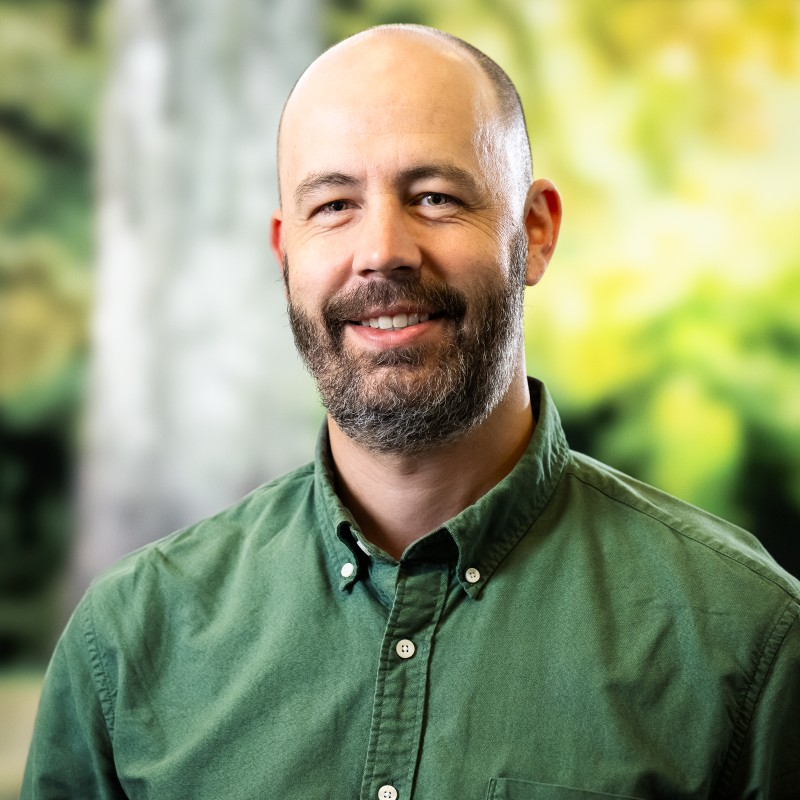
\includegraphics[width=0.75\textwidth]{raffenet.jpg}
			\end{figure}
			\begin{itemize}
				\item {\Large Ken Raffenetti}
				\item \href{mailto:raffenet@anl.gov}{\texttt{raffenet@anl.gov}}
				\item Mathematics and Computer Science
			\end{itemize}
		\end{column}
	\end{columns}
\end{frame}

\subsection{MPICH}
\begin{frame}{MPICH}
	MPICH is a leading MPI implementation and a large open-source project.

	\begin{figure}
		\centering
		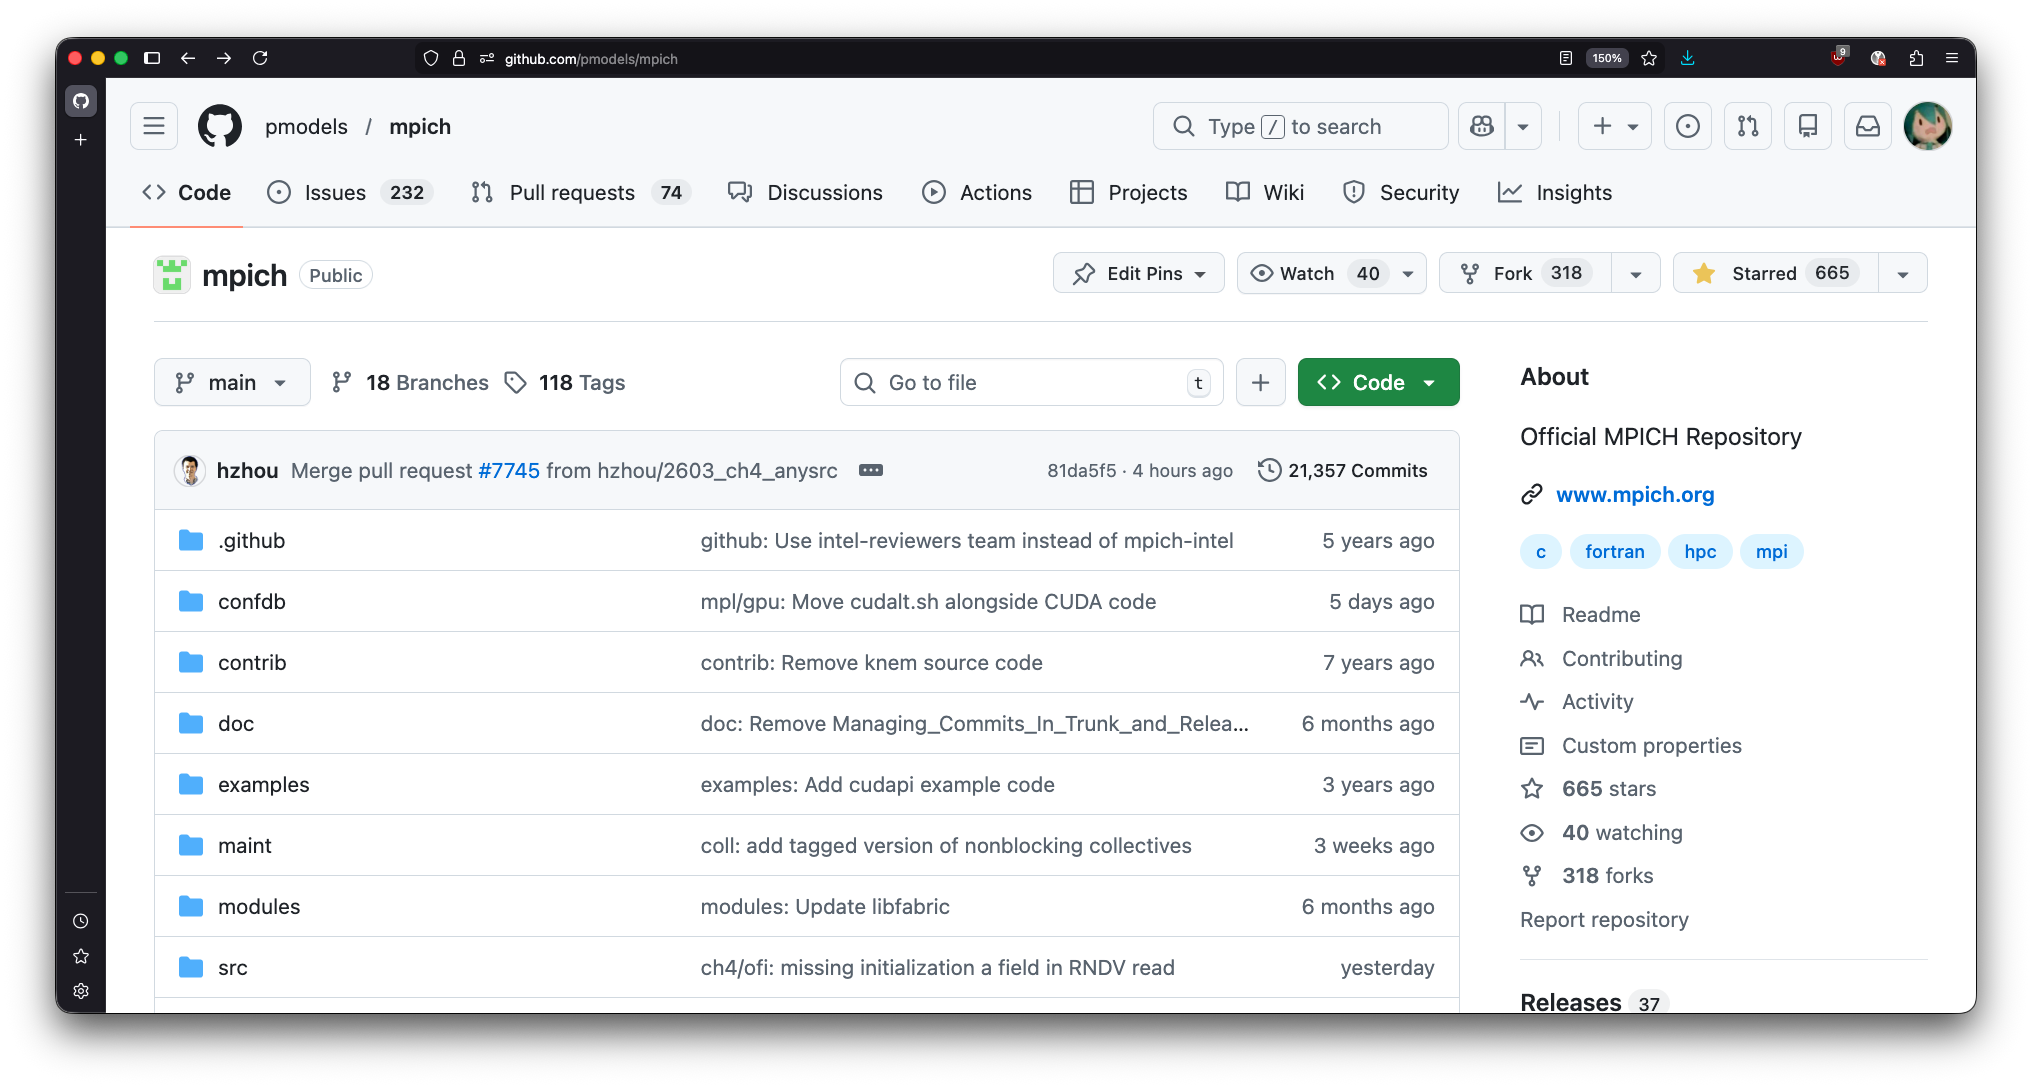
\includegraphics[width=\textwidth]{mpich.png}
		\caption{MPICH GitHub\footnote{\url{github.com/pmodels/mpich}}}
	\end{figure}
\end{frame}

\subsection{Our Maintainer Workflow}
\begin{frame}{Our Maintainer Workflow}
	\begin{columns}
		\begin{column}{0.55\textwidth}
			\begin{figure}
				\centering
				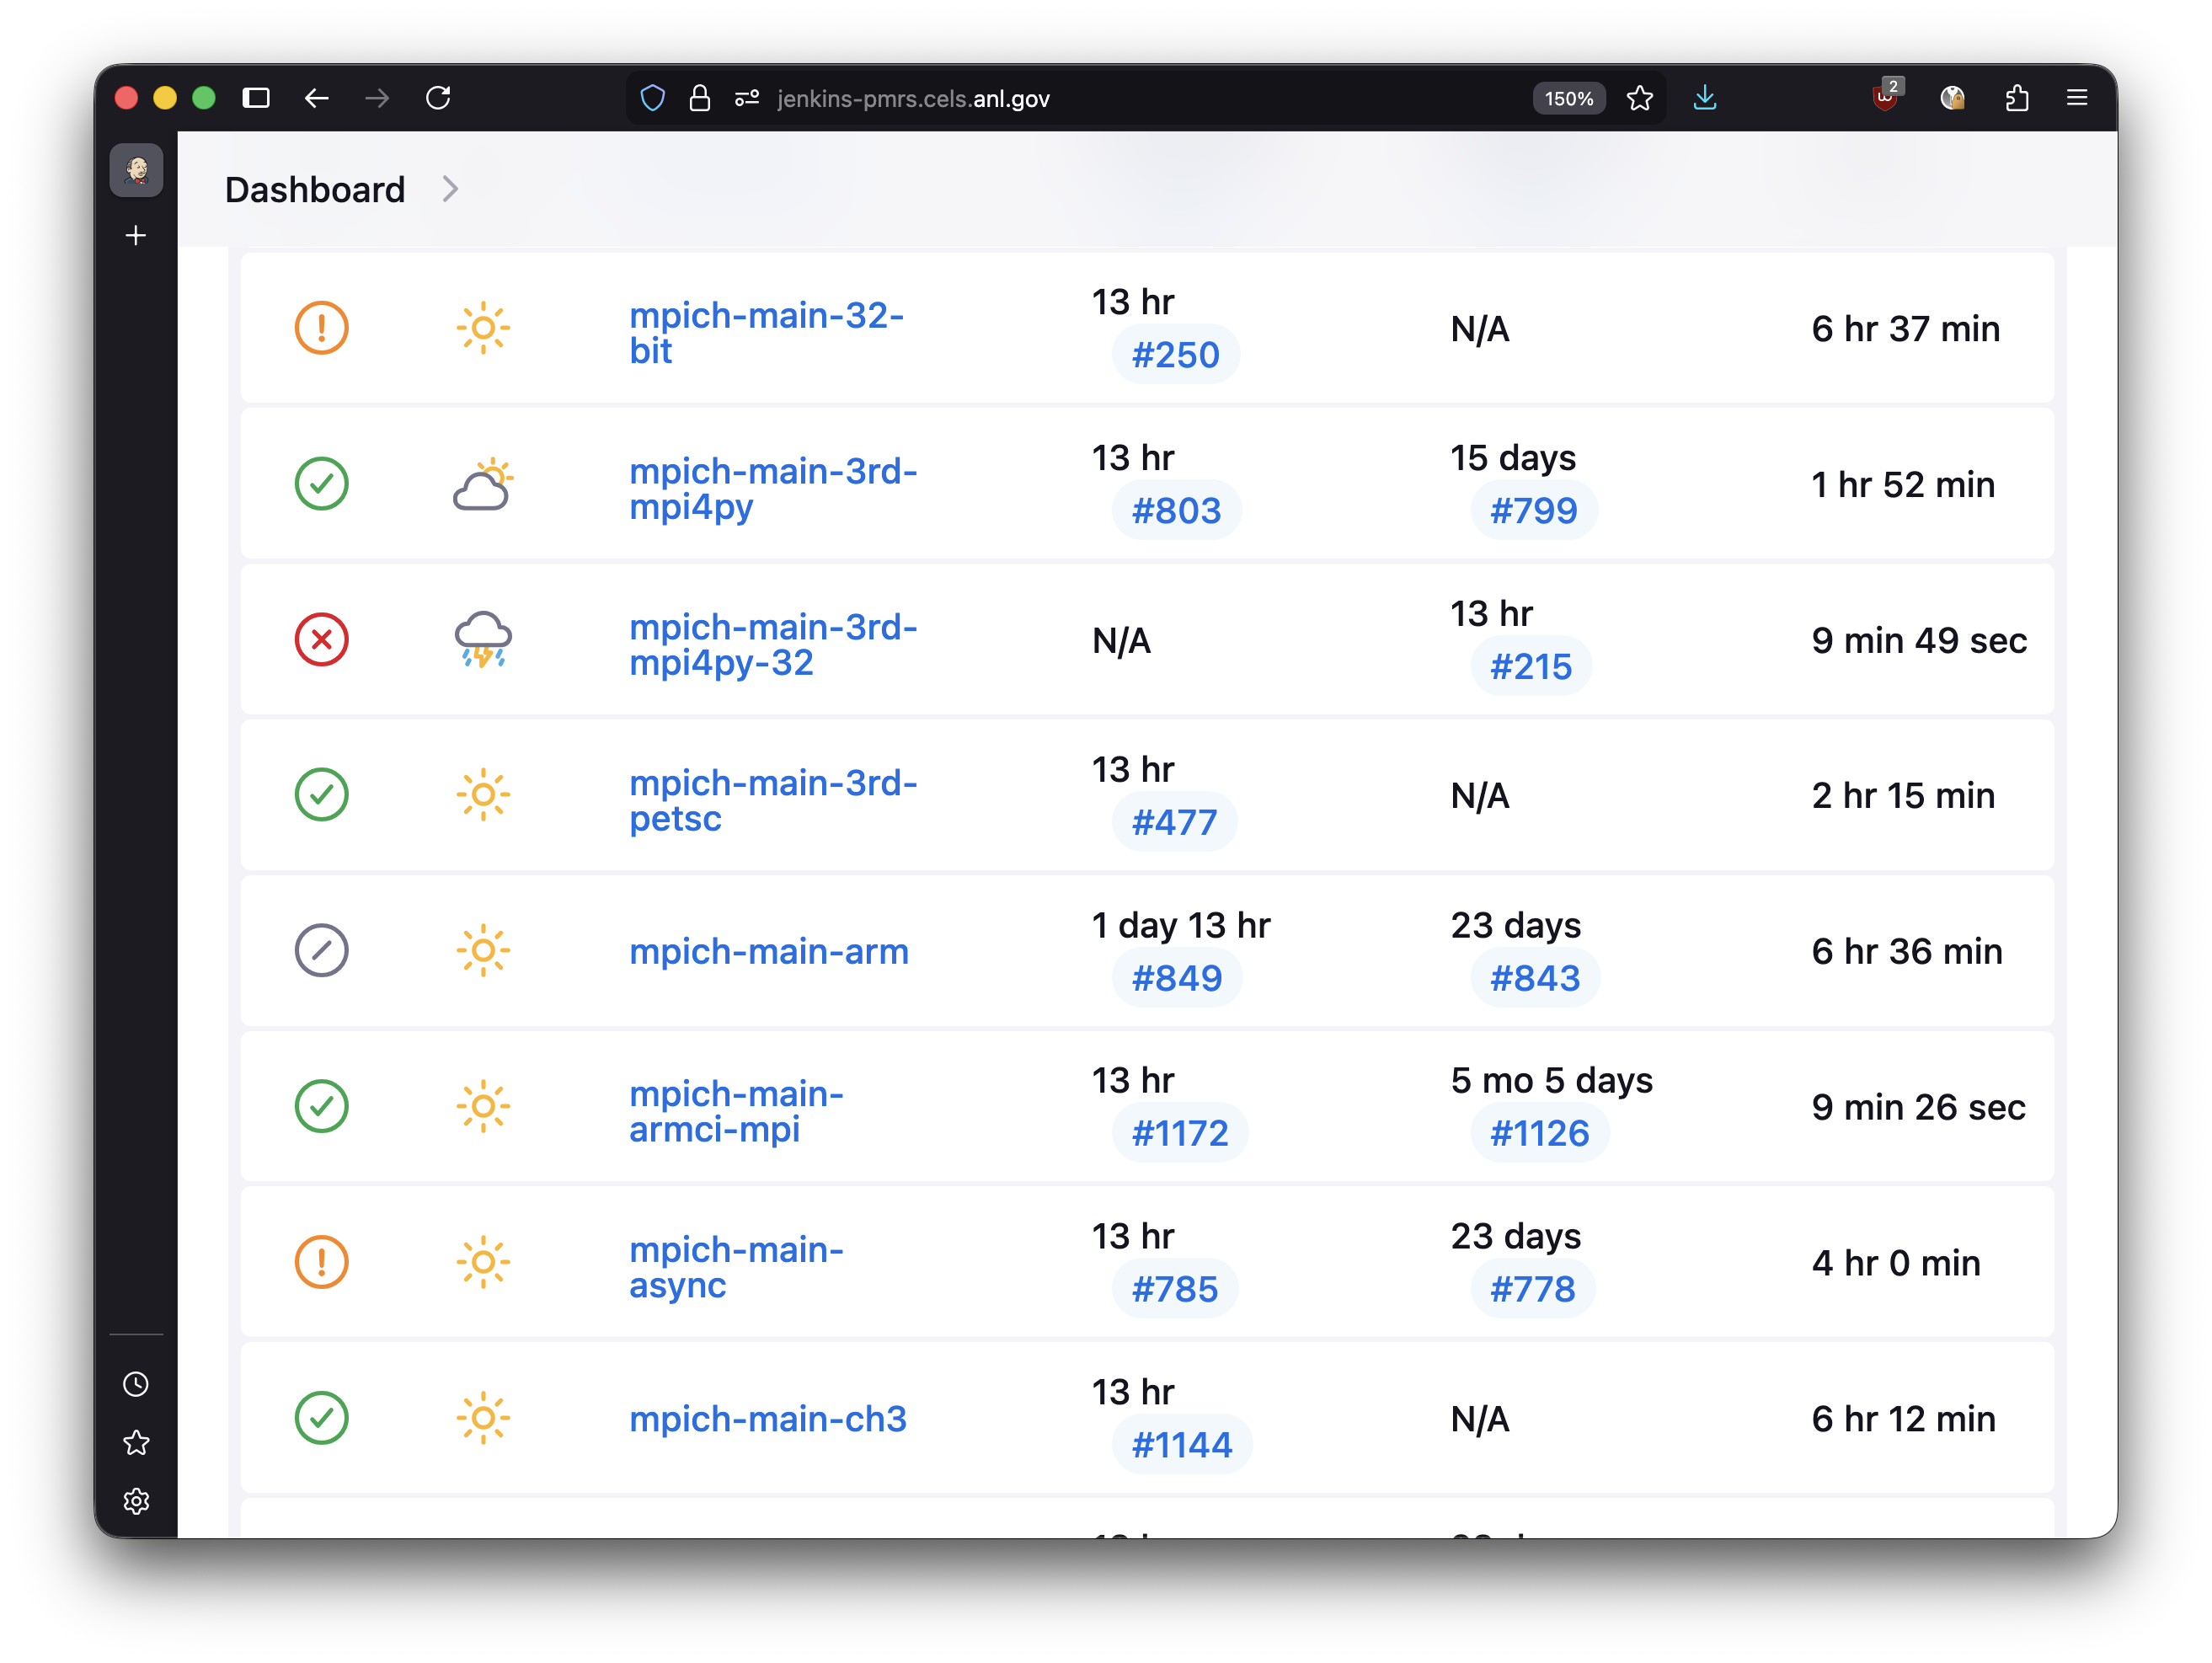
\includegraphics[width=\textwidth]{jenkins.png}
				\caption{PMRS
				Jenkins\footnote{\url{jenkins-pmrs.cels.anl.gov}}}
			\end{figure}
		\end{column}
		\begin{column}{0.45\textwidth}
			CI heavily optimizes our development workflow.
			\pause
			\begin{itemize}
				\item Holistic coverage
					\pause
					\begin{itemize}
						\item Compilers
						\item OS
						\item \texttt{asan}, \texttt{debug}, ...
						\item Async progress
						\item GPU collectives
						\item etc...
					\end{itemize}
					\pause
				\item All PRs test against CI
					\pause
				\item \texttt{main} validated \underline{nightly}
			\end{itemize}
		\end{column}
	\end{columns}
\end{frame}

\begin{frame}{Our Maintainer Workflow}
	\Large
	\begin{align*}
		\text{Nightly Jobs} &\approx 300 \text{ matrix configurations}\\
		&\mapsto N \times M \times ... \text{ combinations}\\
		&\Rightarrow \mathbf{1500} \text{ runs \underline{nightly}}
	\end{align*}
\end{frame}

\begin{frame}{Our Maintainer Workflow}
	\begin{figure}
		\centering
		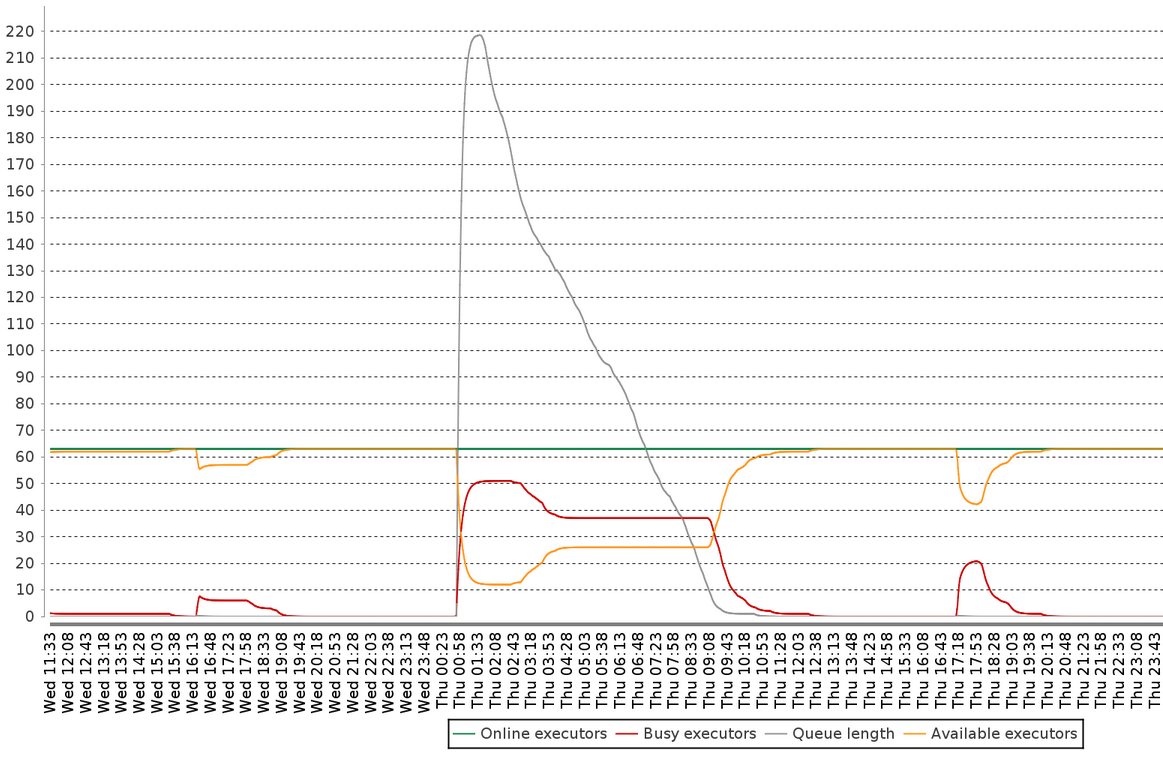
\includegraphics[width=\textwidth]{load-usage.png}
		\caption{Jenkins Load Usage Statistics}
	\end{figure}
\end{frame}

\begin{frame}{Qualms}
	Our CI pipeline is ssslllooooowwwww... :(
	\pause

	\begin{alertblock}{Baseline}
		{\Large \textbf{$\sim$1 hour 30 minutes}}
		\pause
		\textit{per-run}
	\end{alertblock}
	\pause

	\begin{figure}
		\centering
		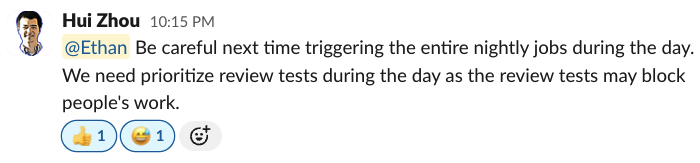
\includegraphics[width=\textwidth]{oops.png}
		\caption{Re-running Nightly Testsuite at 2 PM}
	\end{figure}
\end{frame}

\begin{frame}{Qualms}
	\begin{block}{Per-Run Rebuilds}
		\begin{figure}
			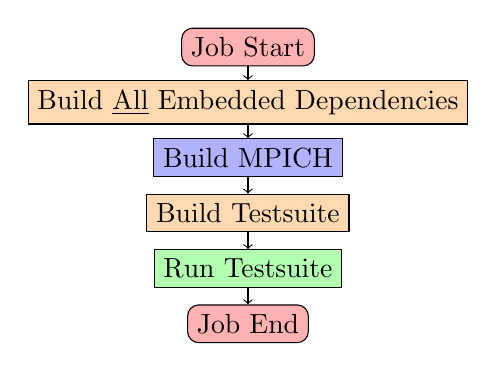
\begin{tikzpicture}[node distance=2em]
				\node (n0) at (0,0) [rectangle, rounded corners, draw=black,
				fill=red!30] {Job Start};
				\node (n1) [rectangle, draw=black, fill=orange!30, below of=n0]
				{Build \underline{All} Embedded Dependencies};
				\node (n2) [rectangle, draw=black, fill=blue!30, below of=n1]
				{Build MPICH};
				\node (n3) [rectangle, draw=black, fill=orange!30, below of=n2]
				{Build Testsuite};
				\node (n4) [rectangle, draw=black, fill=green!30, below of=n3]
				{Run Testsuite};
				\node (n5) [rectangle, rounded corners, draw=black, fill=red!30,
				below of=n4] {Job End};
				\draw [->] (n0) -- (n1);
				\draw [->] (n1) -- (n2);
				\draw [->] (n2) -- (n3);
				\draw [->] (n3) -- (n4);
				\draw [->] (n4) -- (n5);
			\end{tikzpicture}
		\end{figure}
	\end{block}
	\pause

	\begin{itemize}
		\item Builds are reliant on host agents' system packages
			\pause
			\begin{itemize}
				\item Difficult to maintain consistency
				\item Significant effort to test arbitrary versions
			\end{itemize}
	\end{itemize}
	\pause
	$\implies$ \textbf{inflexible}
\end{frame}

\section{Methodology}
\begin{frame}{What Should We Do?}
	This seems like a job for a package manager...
	\pause

	\begin{alertblock}{Spack?}
		\begin{figure}
			\centering
			\includesvg[width=0.25\textwidth]{spack.svg}
		\end{figure}
		\pause

		\begin{enumerate}
			\item Aggressive caching of $n$ build configurations
				\pause
			\item Declarative build/test environments
				\pause
				\begin{itemize}
					\item Explicit \textit{per-package} dependency declaration
						\pause
				\end{itemize}
			\item HPC a first-class citizen
		\end{enumerate}
	\end{alertblock}
\end{frame}

\subsection{Design/Integration}
\begin{frame}{Implementation}
	How should we do this?
	\pause

	\begin{figure}
		\centering
		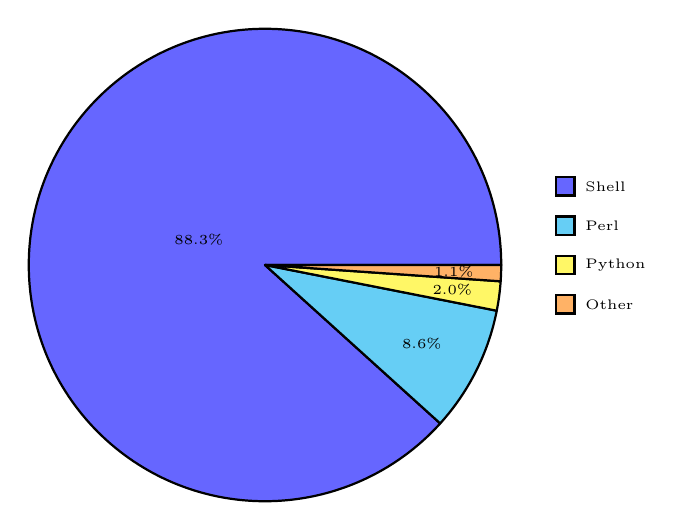
\begin{tikzpicture}
			\tikzstyle{every node}=[font=\tiny]
			\pie[text=legend]{88.3/Shell, 8.6/Perl, 2.0/Python, 1.1/Other}
		\end{tikzpicture}
		\caption{Jenkins Scripts Repository}
	\end{figure}
	\pause

	\underline{Minimal} changes \pause
	$\implies$ \textbf{\textit{Substitute} compilation with Spack!}
\end{frame}

\begin{frame}{Design}
	\begin{alertblock}{Idea}
		Let's treat each component of MPICH as a Spack package.
		\pause
		\begin{figure}
			\centering
			\begin{forest}
				forked edges,
				for tree={grow'=0,draw}
				[MPICH
				[MPL,name=mpl]
				[ROMIO,name=romio]
				[existing \texttt{./configure} opts
				[hwloc]
				[libfabric]
				[ucx]
				[Yaksa,name=yaksa]
				]
				[json-c,name=jsonc]
				[test/mpi]
				]
				\draw[>->] (mpl)--(romio);
				\draw[>->] (jsonc.east)-|-(yaksa);
			\end{forest}
			\caption{MPICH Dependency Graph\footnote{direct dependents}}
		\end{figure}
	\end{alertblock}
\end{frame}

\begin{frame}[fragile]{Design}
	We can easily define an ``Internal PMRS Spack Repository'' with each
	component.
	\pause
	\begin{itemize}
		\item Direct control of MPICH dependencies\footnote{i.e. forked
			versions, cherry-picked patches, etc.}
			\pause
		\item Can soft-fork upstream package definitions
			\pause
	\end{itemize}

	\begin{examples}
		\begin{minted}[fontsize=\tiny]{python3}
from spack_repo.builtin.packages.ucx.package import Ucx as BuiltinUcx
from spack.package import *


class Ucx(BuiltinUcx):
	version(
		"1.19.0-embedded",
		git="https://github.com/pmodels/ucx.git",
		commit="4020d2be2271da0ac105d824f26ec76ad533577a",
	)

	@when("@1.19.0-embedded")
	def autoreconf(self, spec, prefix):
		Executable("./autogen.sh")()
		\end{minted}
	\end{examples}
\end{frame}

\begin{frame}{Design}
	\begin{figure}
		\tiny
		\centering
		\begin{forest}
			for tree={grow'=0,folder,draw}
			[jenkins-scripts/spack\_repo/pmrs/mpich
			[packages
			[hwloc
			[package.py]
			]
			[json\_c
			[package.py]
			]
			[libfabric
			[package.py]
			]
			[mpich
			[package.py]
			]
			[mpich\_testsuite
			[package.py]
			]
			[ucx
			[package.py]
			]
			]
			[repo.yaml]
			]
		\end{forest}
		\caption{Internal PMRS Spack Repository}
	\end{figure}
\end{frame}

\begin{frame}{Integration with Jenkins}
	Our matrix jobs have custom \textit{labels} which correspond to
	\texttt{./configure} options.

	\begin{examples}
		\begin{figure}
			\centering
			\begin{tabular}{ |c|c|c| }
				\hline
				\textbf{Configuration Matrix} & \textbf{gnu} & \textbf{clang} \\
				\hline
				\texttt{ch3-tcp} & \checkmark & \checkmark \\
				\hline
				\texttt{ch3-sock} & \checkmark & \checkmark \\
				\hline
				\texttt{ch4-ofi} & \checkmark & \checkmark \\
				\hline
			\end{tabular}
			\caption{\texttt{mpich-main-osx}\footnote{\url{jenkins-pmrs.cels.anl.gov/job/mpich-main-osx}}
			CI Job}
		\end{figure}
	\end{examples}
	\pause

	How do we translate these to \texttt{spack install}s?
\end{frame}

\begin{frame}{Integration with Jenkins}
	\begin{figure}
		\centering
		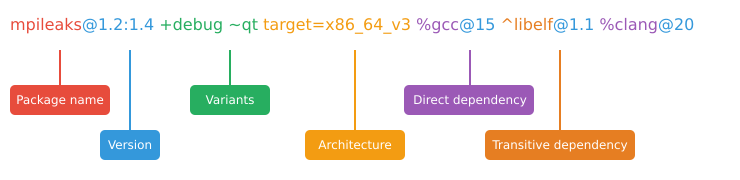
\includegraphics[width=\textwidth]{spec_anatomy.png}
		\caption{Spec Syntax\footnote{\url{spack.readthedocs.io/en/latest/spec\_syntax.html}}}
	\end{figure}

	\begin{alertblock}{Idea}
		Let's generate equivalent Spack specs!
		\pause
		\begin{itemize}
			\item Reuse $\text{Label} \mapsto \text{\texttt{./configure}
				option}$ mappings
				\pause
			\item Variants provide configuration granularity
				\pause
			\item Dependencies can be explicitly resolved
		\end{itemize}
	\end{alertblock}
\end{frame}

\begin{frame}{Integration with Jenkins}
	\begin{examples}
		\small{\texttt{config\_opt=' --with-device=\textbf{ch4:ofi}
		--\textbf{without-xpmem} --with-wrapper-dl-type=\textbf{rpath}
		--with-hwloc=\textbf{embedded} --with-libfabric=\textbf{embedded}'}}
		\pause

		\begin{equation*}
			\Big\Downarrow
		\end{equation*}

		\small{\texttt{mpich@develop device=\textbf{ch4} netmod=\textbf{ofi}
		\textbf{\~{}xpmem} wrapper-dl-type=\textbf{rpath} \textbf{+hwloc}
		\%hwloc@2.9.0-\textbf{embedded} \%libfabric@1.20.1-\textbf{embedded}}}
	\end{examples}
	\pause

	\begin{alertblock}{Idea++}
		We can generalize this to a tool which templates Spack
		specs/environments for our CI\footnote{and for us maintainers} to
		concretize and install.
	\end{alertblock}
\end{frame}

\begin{frame}{PR Jobs}
	We can also utilize \texttt{spack develop} and \texttt{@<sha-1>} Git
	versions to validate contributed PRs \textit{while utilizing Spack}!
	\pause

	\begin{examples}
		\begin{figure}
			\centering
			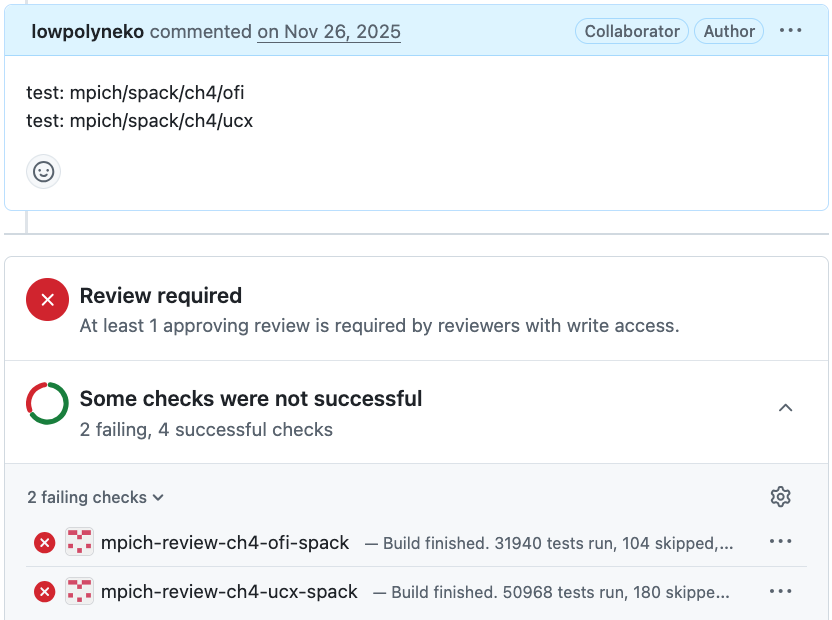
\includegraphics[width=0.55\textwidth]{pr.png}
			\caption{Example PR Utilizing Spackified CI
			Jobs\footnote{\tiny\url{jenkins-pmrs.cels.anl.gov/job/mpich-review-ch4-ofi-spack}}\footnote{\tiny\url{jenkins-pmrs.cels.anl.gov/job/mpich-review-ch4-ucx-spack}}}
		\end{figure}
	\end{examples}
\end{frame}

\subsection{Bug!}
\begin{frame}{Concurrent Jobs}
	An interesting consequence of integrating Spack into our existing CI
	infrastructure is that per-job \texttt{spack install}s run in parallel.
	\pause

	\begin{examples}
		\begin{figure}
			\small
			\centering
			\begin{forest}
				[Jenkins
				[\texttt{pmrs-linux-01}
				[\texttt{mpich-main-gpu}
				[ucx]
				[hwloc]
				]
				]
				[\texttt{pmrs-linux-02}
				[\texttt{mpich-review-ofi}
				[libxml2]
				[libfabric]
				]
				]
				[\texttt{pmrs-macos-01}
				[\texttt{mpich-main-osx}
				[json-c]
				]
				]
				]
			\end{forest}
		\end{figure}
	\end{examples}
	\pause

	\begin{block}{Bug!}
		We ran into a race condition with Spack's installer...
	\end{block}
\end{frame}

\begin{frame}{Concurrent Jobs}
	\begin{figure}
		\centering
		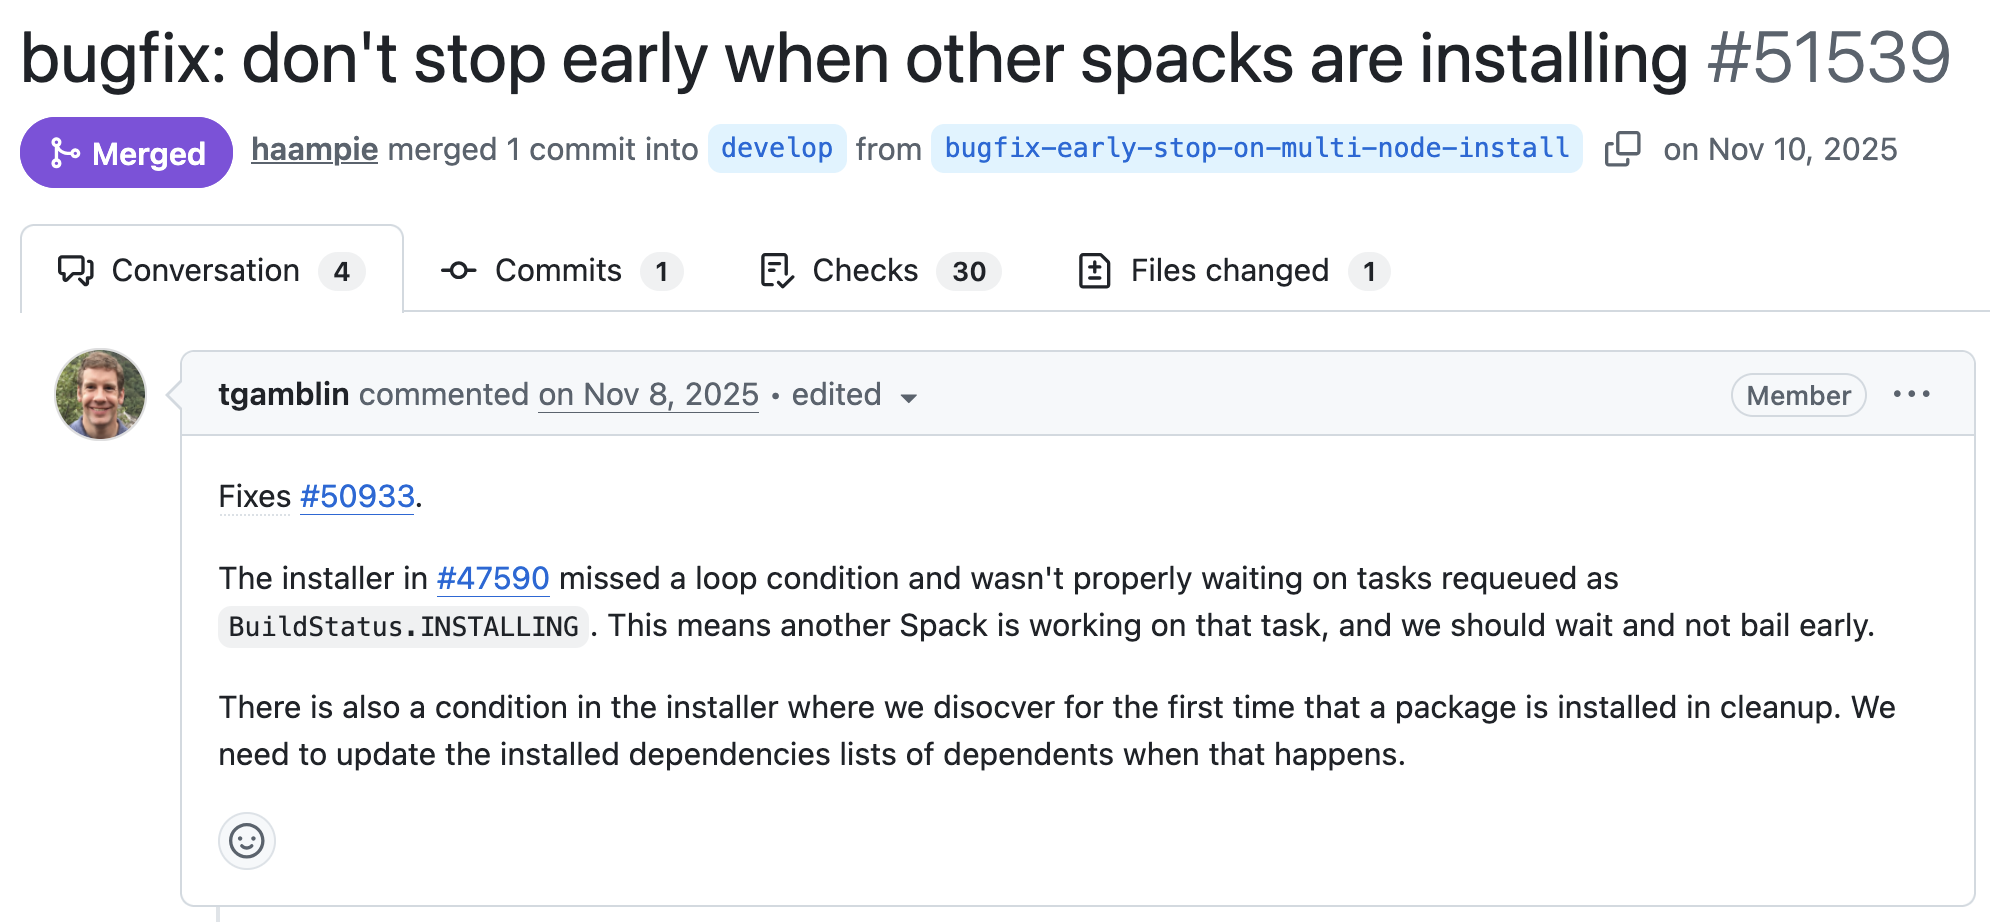
\includegraphics[width=\textwidth]{bug.png}
		\caption{\url{github.com/spack/spack/pull/51539}}
	\end{figure}
	\pause

	Thank you, Todd!
\end{frame}

\section{Results}
\begin{frame}{Results}
	On average, our CI builds are now \textbf{$33\%$ faster!}
	\pause
	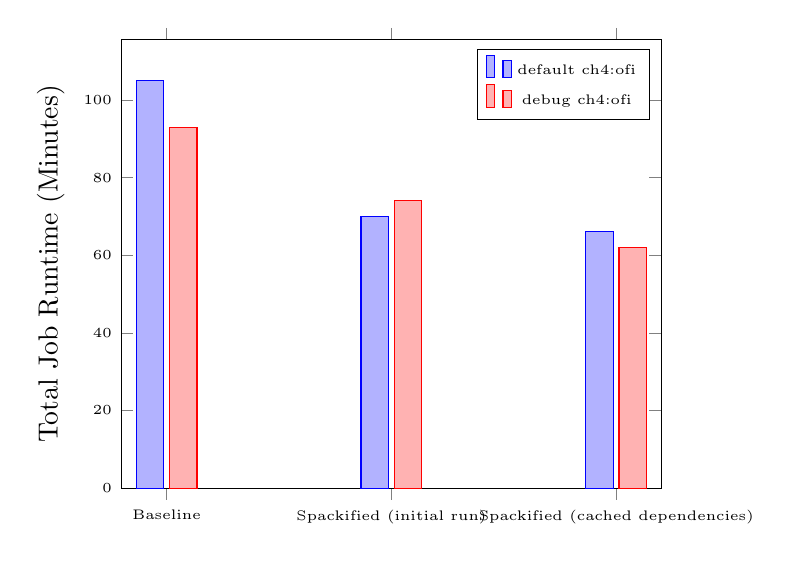
\begin{tikzpicture}
		\begin{axis}[
			ybar,
			ymin=0,
			ylabel={Total Job Runtime (Minutes)},
			symbolic x coords={Baseline,Spackified (initial run),Spackified
			(cached dependencies)},
			xtick=data,
			ticklabel style={font=\tiny},
			legend style={font=\tiny}
			]
			\addplot coordinates {(Baseline,105) (Spackified (initial run),70)
			(Spackified (cached dependencies),66)};
			\addplot coordinates {(Baseline,93) (Spackified (initial run),74)
			(Spackified (cached dependencies),62)};
			\legend{default ch4:ofi,debug ch4:ofi}
		\end{axis}
	\end{tikzpicture}\\
	\pause
	The primary bottleneck now is our \underline{single-threaded testsuite}.
\end{frame}

\begin{frame}{Results++}
	As maintainers, we also benefit from massive QoL boosts!
	\pause
	\begin{itemize}
		\item We can pull any MPICH build from the Spack install cache, prebuilt
			by our CI
			\pause
		\item We have cleanroom\footnote{-ish} environments for our CI jobs
			\pause
		\item External dependencies now build independently of MPICH
			\pause
		\item For \textit{matrix configurations}, we now cache identical builds
	\end{itemize}
\end{frame}

\section{Closing Remarks}
\subsection{Future Work}
\begin{frame}{Future Work}
	We see huge potential in further integration of Spack for our CI.
	\pause

	\begin{block}{Our Ideas}
		\begin{itemize}
			\item Refactoring internal, embedded modules to be cachable by Spack
				\pause
				\begin{itemize}
					\item MPL
					\item ROMIO
					\item etc...
				\end{itemize}
				\pause
			\item Pre-compilation of our entire testsuite
				\pause
			\item Try integrating \texttt{ccache} for better compilation
				granularity
				\pause
			\item Mirroring of CI builds for public usage
				\pause
			\item Exporting test environment as OCI images?
				\pause
		\end{itemize}
	\end{block}

	The future is bright for our CI! \^{}w\^{}
\end{frame}

\begin{frame}{Recap}
	\tableofcontents
\end{frame}

\begin{frame}{Closing Remarks}
	\begin{center}
		{\Huge Thank you!}

		\begin{itemize}
			\item Hopefully this inspires other projects to attempt a similar
				endeavor.
			\item \textit{We'll stick around to chat afterwards...}
		\end{itemize}
	\end{center}
\end{frame}

\end{document}

% vim: tw=80:ts=4:sw=4:noexpandtab:spell:
